\documentclass[]{beamer} 
\setbeamerfont{all}{size=\large}
\setbeamerfont*{itemize/enumerate body}{size=\large}
\setbeamerfont*{itemize/enumerate subbody}{parent=itemize/enumerate body}
\setbeamerfont*{itemize/enumerate subsubbody}{parent=itemize/enumerate body}
\beamertemplatenavigationsymbolsempty
\usetheme{default}
\useinnertheme{circles}
\usebeamerfont{all}
\DeclareMathOperator*{\argmin}{arg\,min}
\usepackage{listings}
\usepackage{amssymb}
\usepackage{docmute}
\usepackage{hyperref}
\begin{document}

%\hspace*{\fill} \\

\title{Faster Image Segmentation with ENet}
\author{Nicholas Dronen}

\begin{frame}
\maketitle
\end{frame}

%\input{01-inception}
%\input{02-enet}
%\input{03-distillation}

\begin{frame}
\centering
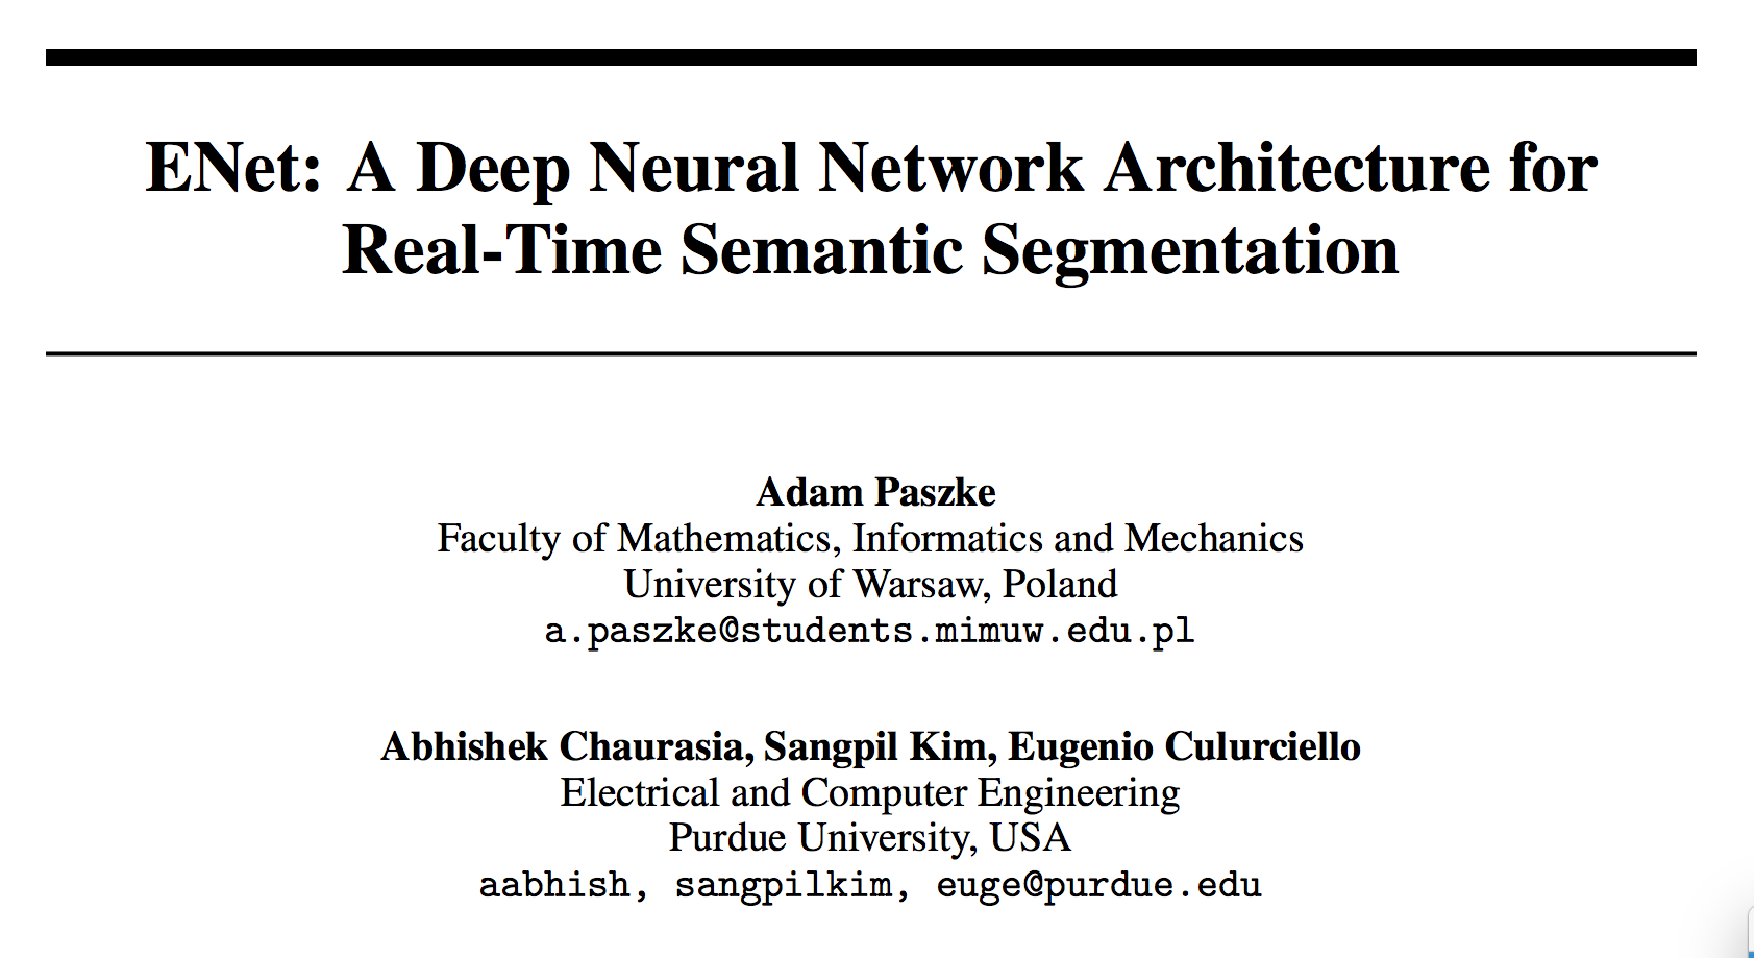
\includegraphics[width=0.9\textwidth]{figures/enet-title} \\
\href{https://arxiv.org/abs/1606.02147}{\textcolor{blue}{arXiv:0706.1234v1 [cs.CV]}}
\end{frame}

\begin{frame}{ENet versus SegNet: Inference Speed}
\centering
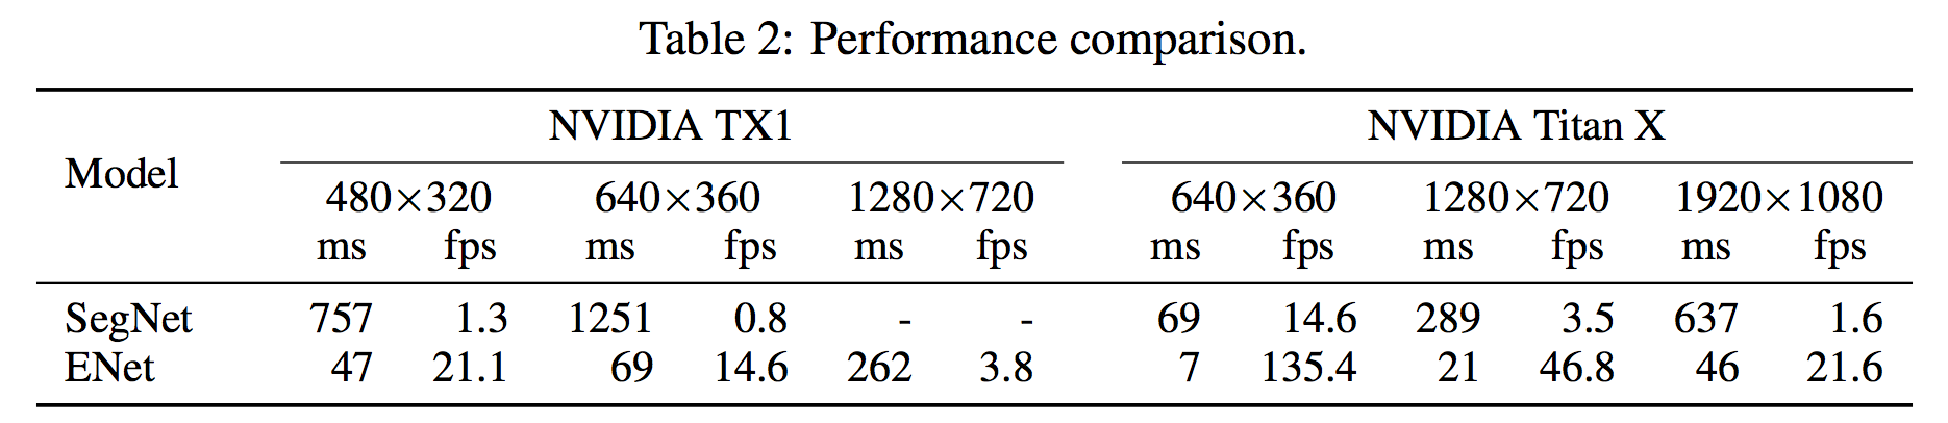
\includegraphics[width=0.9\textwidth]{figures/enet-vs-segnet-speed} \\
\hspace*{\fill} \\
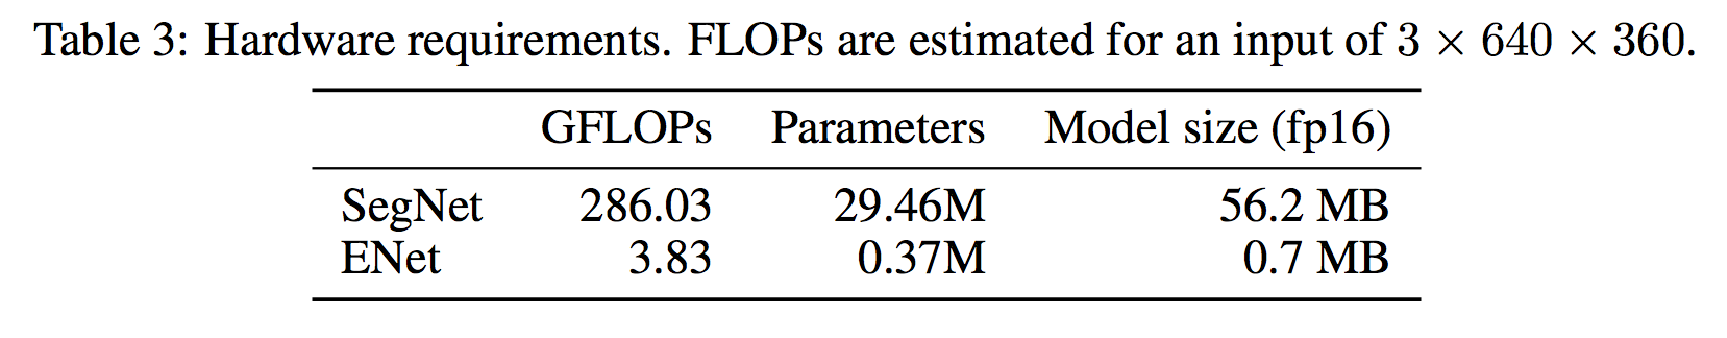
\includegraphics[width=0.9\textwidth]{figures/enet-vs-segnet-gflops-size}
\end{frame}

\begin{frame}{ENet versus SegNet: Model Accuracy}
\centering
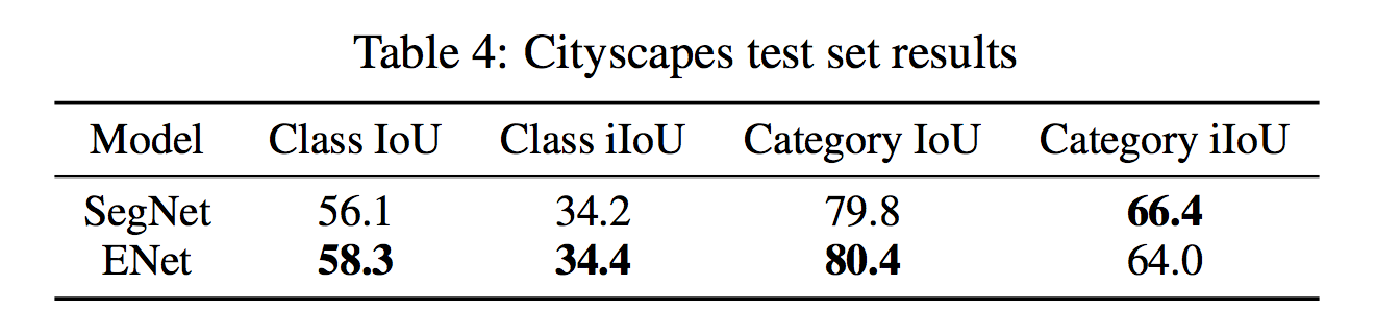
\includegraphics[scale=0.325]{figures/enet-versus-segnet-accuracy-1-cityscapes} \\
\hspace*{\fill} \\
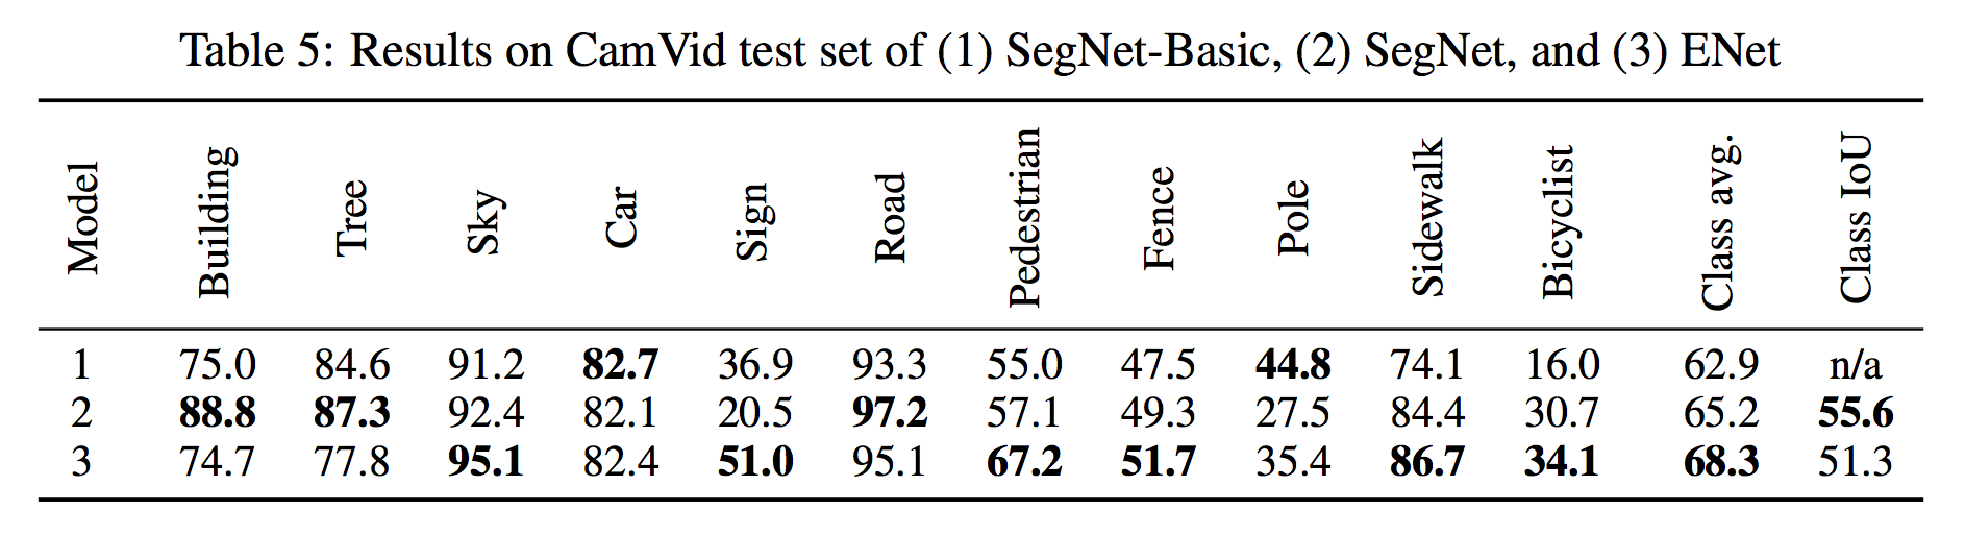
\includegraphics[scale=0.325]{figures/enet-versus-segnet-accuracy-2-camvid} \\
\hspace*{\fill} \\
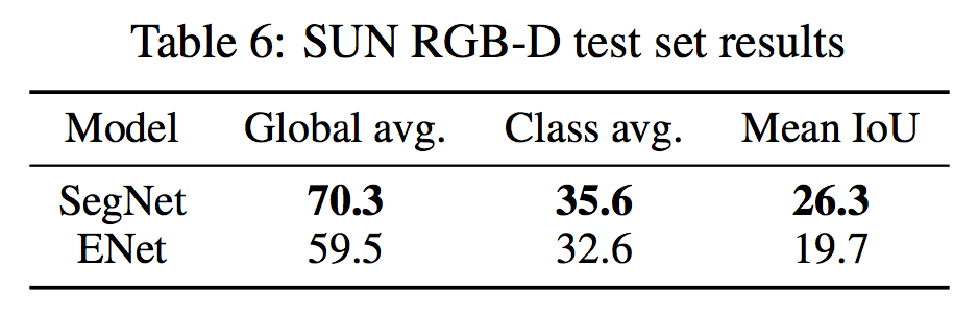
\includegraphics[scale=0.325]{figures/enet-versus-segnet-accuracy-3-sun-rgbd} \\
\end{frame}

\begin{frame}{$1 \times 1$ Convolutions}
\centering
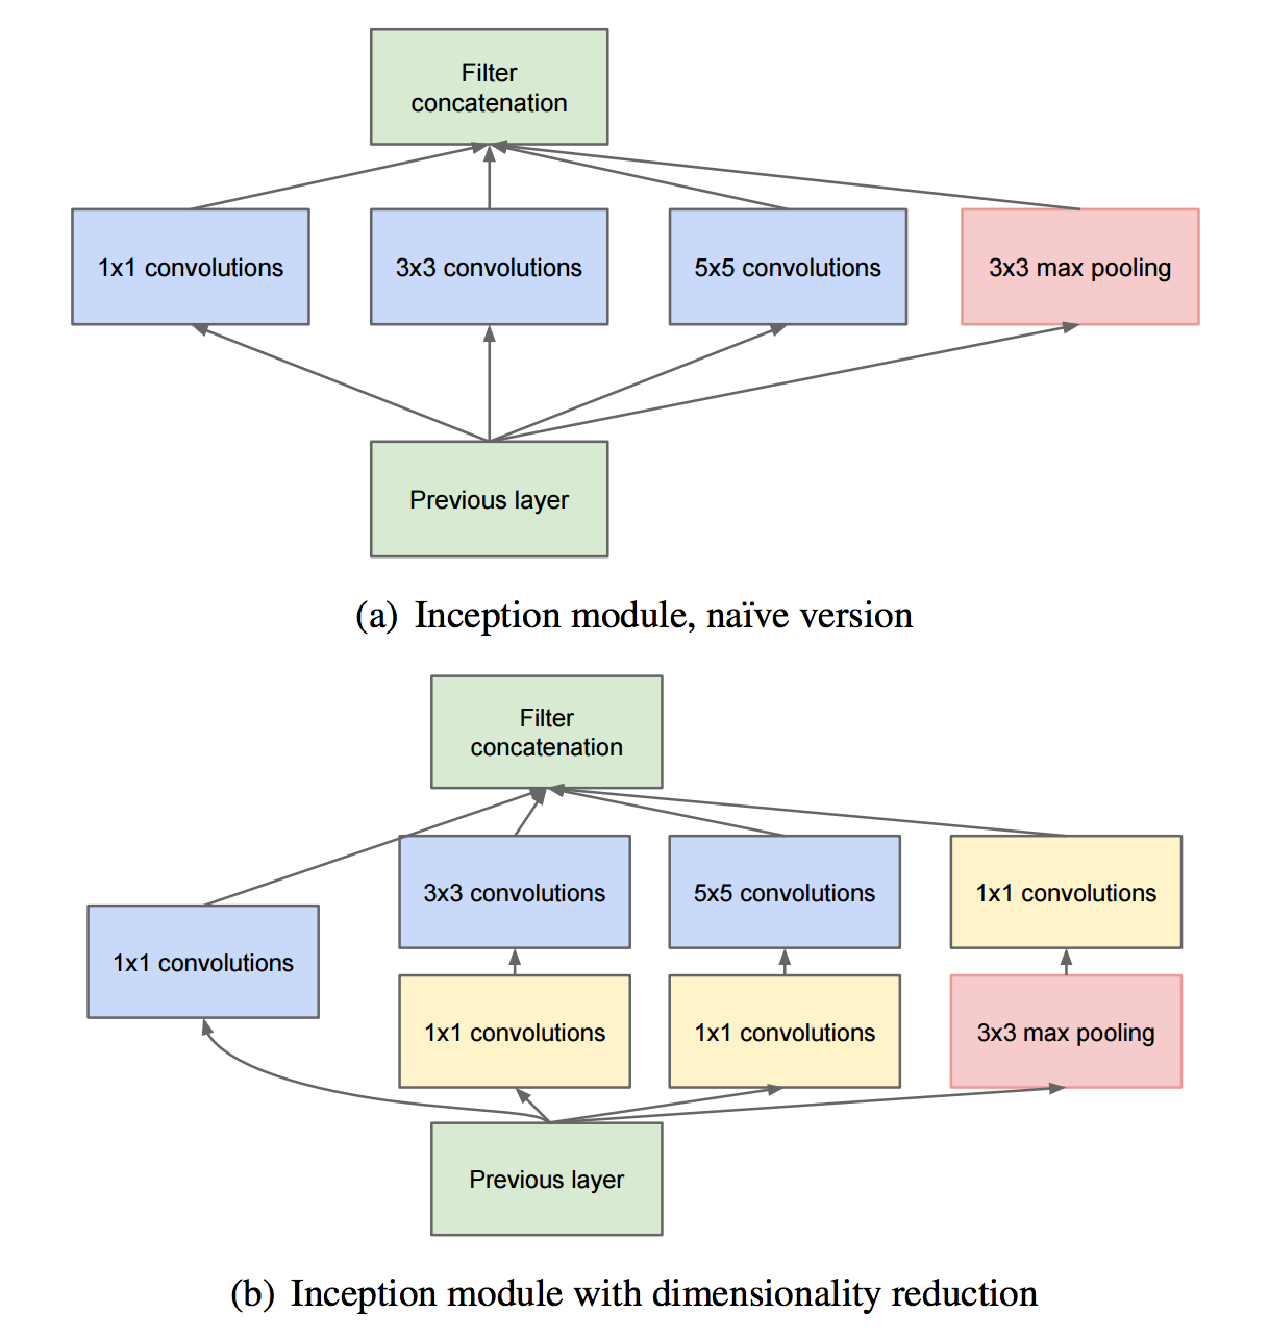
\includegraphics[scale=0.375]{figures/1x1-convolutions}
\end{frame}

\end{document}

%\begin{frame}[fragile]{}
%\begin{lstlisting}
% Verbatim code goes here.
%\end{lstlisting}
%\end{frame}

